\label{sec:empirical}
In this section, we present some empirical observations that either verifies, or are induced by the decoupling conjecture.
We conduct experiments on the CIFAR-10, CIFAR-100  \citep{Krizhevsky09learningmultiple}, and MNIST  \citep{lecun1998gradient} datasets as well as their random labeled versions, namely MNIST-R and CIFAR10-R. 
% We use PyTorch \citep{NEURIPS2019_9015} framework for all experiments.
We used different fully connected (fc) networks (a fc network with $m$ hidden layers and $n$ neurons each hidden layer is denoted as F-$n^m$), several variations of LeNet \citep{lecun1998gradient}, VGG11 \citep{simonyan2014very}, and ResNet18 \citep{kaiming2015}.
% The results shown in the main text are from variants of VGG11 and ResNet18 trained on CIFAR100, variants of LeNet5 trained on CIFAR10, and F-$200^2$ trained on MNIST.
% The eigenvalues and eigenvectors of the exact layer-wise Hessians are approximated using a modified Lanczos algorithm \citep{hessian-eigenthings} which is described in detail in \sectionref{sec:appendix_eigencomp}. 
We use ``layer:network'' to denote a layer of a particular network. For example, conv2:LeNet5 refers to the second convolutional layer in LeNet5.
More empirical results are included in \sectionref{sec:appendix_exp_res}.

\subsection{Kronecker Approximation of Layer-wise Hessian and Full Hessian}\label{subsec:approx}

% \begin{figure}[h]
% \centering
% \vspace{-1em}
% \subfigure[\small{Top eigenvalues of\\ $\mH_\cL^{(i)}$ and $\hat\mH_\cL^{(i)}$ (fc1)}]{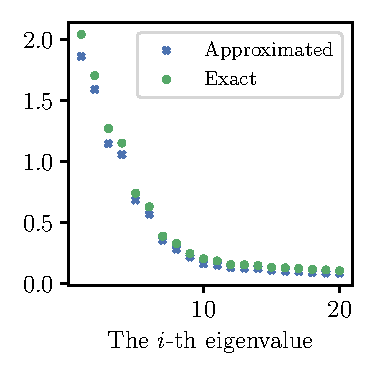
\includegraphics[width=0.24\linewidth]{Figures/ApproxQuality/FC2_fixlr/eigenval_compare_top20_MNIST_Exp1_FC2_fixlr0.01R2_E-1_narrow_fc1.pdf}}
% \subfigure[\small{Eigenspace overlap\\ of $\hat\mH^{(i)}_\cL$ and $\mH^{(i)}_\cL$}]{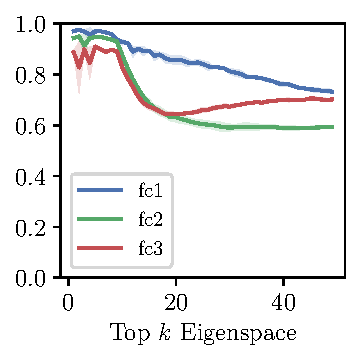
\includegraphics[width=0.24\linewidth]{Figures/ApproxQuality/FC2_fixlr/sample_kron_decomp_traceoverlap_d80_MNIST_Exp1_FC2_fixlr0.01Average_E-1_narrow.pdf}}
% \subfigure[\small{Top eigenvalues of\\ $\mH_\cL$ and $\hat\mH_\cL$ (full)}]{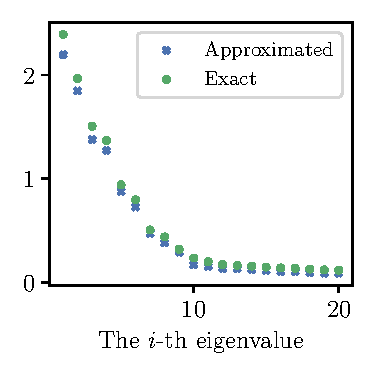
\includegraphics[width=0.24\linewidth]{Figures/ApproxQuality/FC2_fixlr/MNIST_Exp1_FC2_fixlr0.01_fulleigenval_approx.pdf}}
% \subfigure[\small{Eigenspace overlap\\ of $\hat\mH_\cL$ and $\mH_\cL$}]{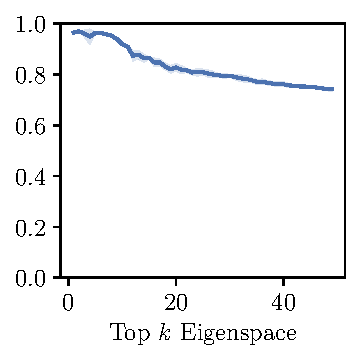
\includegraphics[width=0.24\linewidth]{Figures/ApproxQuality/FC2_fixlr/MNIST_Exp1_FC2_fixlr0.01_Average_fulleigenvec_overlap.pdf}}
% \caption{Comparison between the approximated and true layer-wise Hessian of F-$200^2$. $\mH^{(i)}_\cL$ denote the layer-wise Hessian, and $\mH_\cL$ denote the full Hessian including off-diagonal blocks. The approximated full Hessian $\hat\mH_\cL$ is defined in \sectionref{sec:appendix_full_hessian}}
% \label{fig:eigeninfo_approx}
% \vspace{-1em}
% \end{figure}

% To verify our approximation using Kronecker factorization, we compare the top eigenvalues and eigenspaces of the approximated Hessian and the true Hessian. We use the standard definition of subspace overlap (\cref{def:overlap}) to measure the similarity between top eigenspaces. %We define the dimension $k$ top eigenspace of a matrix as the subspace spanned by the eigenvectors corresponding to its $k$ largest eigenvalues. 
To verify the decoupling conjecture in practical settings, we compare the top eigenvalues and eigenspaces of the approximated Hessian and the true Hessian. We use subspace overlap (\definitionref{def:overlap}) to measure the similarity between top eigenspaces. As shown in \figureref{fig:eigeninfo_approx}, this approximation works reasonably well on the top eigenspace.

\begin{figure}[ht]
    \centering
\begin{subfigure}[b]{0.24\columnwidth}
    \captionsetup{justification=centering}
    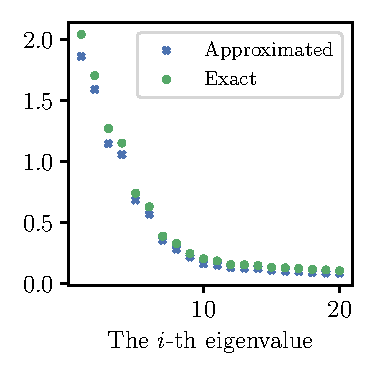
\includegraphics[width=\columnwidth]{Figures/ApproxQuality/FC2_fixlr/eigenval_compare_top20_MNIST_Exp1_FC2_fixlr0.01R2_E-1_narrow_fc1.pdf}
    \vspace{-0.2in}
    \caption{Top eigenvalues of layer-wise Hessian of fc1}
    % \caption{Eigenvalues}
    \label{fig:eigenval_approx}
\end{subfigure}%
\begin{subfigure}[b]{0.24\columnwidth}
    \captionsetup{justification=centering}
    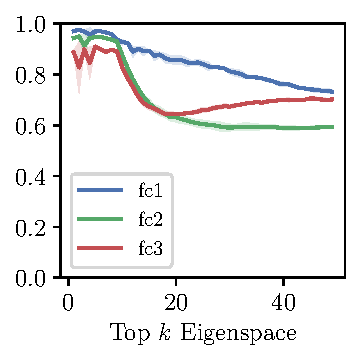
\includegraphics[width=\columnwidth]{Figures/ApproxQuality/FC2_fixlr/sample_kron_decomp_traceoverlap_d80_MNIST_Exp1_FC2_fixlr0.01Average_E-1_narrow.pdf}
    \vspace{-0.2in}
    \caption{Top eigenspace of layer-wise Hessians}
    % \caption{Eigenspace overlap}
    \label{fig:overlap_approx}
\end{subfigure}
\begin{subfigure}[b]{0.24\columnwidth}
    \captionsetup{justification=centering}
    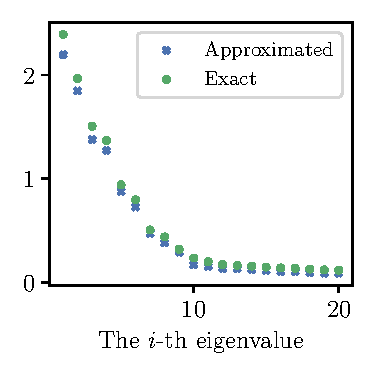
\includegraphics[width=\columnwidth]{Figures/ApproxQuality/FC2_fixlr/MNIST_Exp1_FC2_fixlr0.01_fulleigenval_approx.pdf}
    \vspace{-0.2in}
    \caption{Top eigenvalues of the full Hessian}
    % \caption{Eigenspace overlap}
    \label{fig:eigenval_approx_full}
\end{subfigure}
\begin{subfigure}[b]{0.24\columnwidth}
    \captionsetup{justification=centering}
    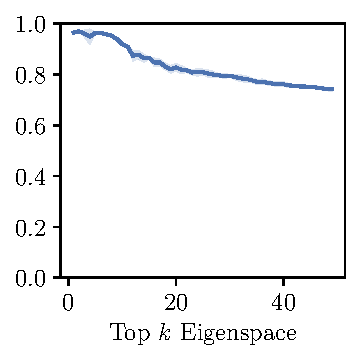
\includegraphics[width=\columnwidth]{Figures/ApproxQuality/FC2_fixlr/MNIST_Exp1_FC2_fixlr0.01_Average_fulleigenvec_overlap.pdf}
    \vspace{-0.2in}
    \caption{Top eigenspace of the full Hessian}
    % \caption{Eigenspace overlap}
    \label{fig:overlap_approx_full}
\end{subfigure}
% \vspace{-0.2in}
\caption{Comparison between the approximated and true layer-wise Hessian of F-$200^2$.}
\vspace{-4pt}
\label{fig:eigeninfo_approx}
\end{figure}
%for the top eigenvalues and eigenspaces of both layer-wise weight Hessians and the full parameter Hessian.
%In this section we leverage the Kronecker factorization to understand structures of the dominating eigenspace of layerwise Hessians.
\subsection{Low Rank Structure of \texorpdfstring{$\E[\mM]$}{EM} and \texorpdfstring{$\mH$}{H}}
\label{sec:emp_outlier}
Another way to empirically verify the decoupling conjecture is to show the similarity between the outliers in eigenspectrum of the layer-wise Hessian $\E[\mM]$ and the output Hessian $\mH_\cL$.
%We can also conjecture that the outliers also appear in $\E[\mM]$.
\figureref{fig:UTAU_H_spec} shows the similarity of eigenvalue spectrum between $\E[\mM]$ and layer-wise Hessians in different situations, which agrees with our prediction. For (a) and  (b) we are also seeing the eigengap at $c-1$, which is consistent with our analysis and previous observations \citep{sagun2017empirical,papyan2019measurements}. However, the eigengap does not appear at minimum for random labeled data with a under-parameterized network, meaning that our theory may not generalize to all settings.

\begin{figure*}[h]
\resizebox{\textwidth}{!}{%
    \centering
    \captionsetup[sub]{format=subcaptionformat}
    \begin{subfigure}[b]{0.3\textwidth}
        \centering
        \captionsetup{justification=centering}
        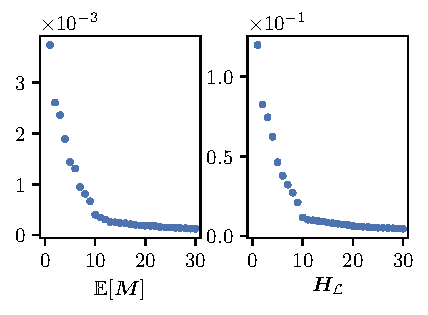
\includegraphics[width=\textwidth]{Figures/EM_vs_H/LeNet5_fixlr_0.01_init/UTAU_vs_full_sigval_d30_CIFAR10_Exp1_LeNet5_fixlr0.01R1_E0_fc1.pdf}
        \caption{fc1:LeNet5 at initialization (CIFAR10).}
        \label{fig:UTAU_H_spec_FC2}
    \end{subfigure}%
    \begin{subfigure}[b]{0.3\textwidth}
        \centering
        \captionsetup{justification=centering}
        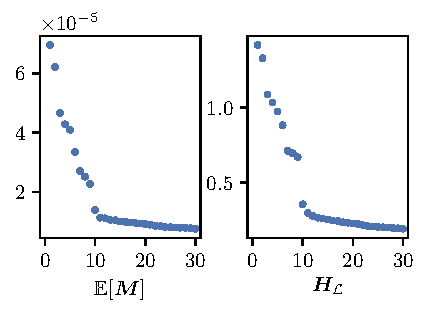
\includegraphics[width=\textwidth]{Figures/EM_vs_H/LeNet5_fixlr0.01/UTAU_vs_full_sigval_d30_CIFAR10_Exp1_LeNet5_fixlr0.01R1_E-1_fc1.pdf}
        \caption{fc1:LeNet5 at minimum\\ (CIFAR10).}
        \label{fig:UTAU_H_spec_Lenet}
    \end{subfigure}%
    \begin{subfigure}[b]{0.3\textwidth}
        \centering
        \captionsetup{justification=centering}
        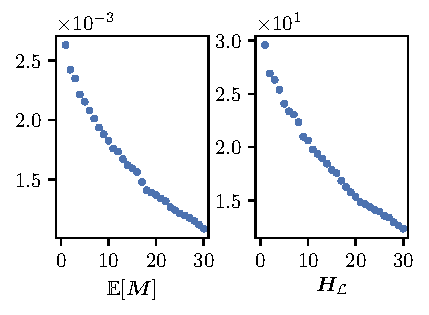
\includegraphics[width=\textwidth]{Figures/EM_vs_H/LeNet5_RL/UTAU_vs_full_sigval_d30_CIFAR10_RandomLabel_LeNet5_fixlr0.01_RLR4_E-1_fc1.pdf}
        \caption{fc1:LeNet5 at minimum\\ (CIFAR10-R).}
        \label{fig:UTAU_H_spec_RL}
    \end{subfigure}%
    }
     %\captionsetup{justification=centering}
    
    \caption{Eigenspectrum of the layer-wise output Hessian $\E[\mM]$ and the layer-wise weight Hessian $\mH_\Ls(\vw^{(p)})$. The vertical axes denote the eigenvalues. Similarity between the two eigenspectra is a direct consequence of a low rank $\E[\vx\vx^T]$ and the decoupling conjecture.}
    \label{fig:UTAU_H_spec}
    \vskip -0.05in
\end{figure*}

% \begin{figure}[h]
%     \centering
%     % \vspace{-1em}
%     \subfigure[\small{fc1:LeNet5 at init\\ (CIFAR10)}]{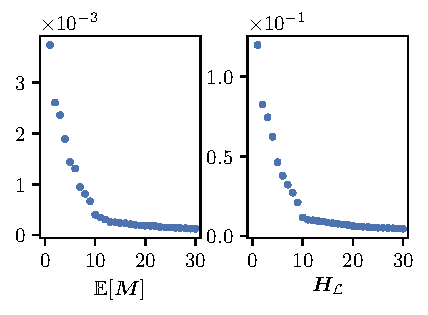
\includegraphics[width=0.25\linewidth]{Figures/EM_vs_H/LeNet5_fixlr_0.01_init/UTAU_vs_full_sigval_d30_CIFAR10_Exp1_LeNet5_fixlr0.01R1_E0_fc1.pdf}}
%     \qquad
%     \subfigure[\small{fc1:LeNet5 at min\\ (CIFAR10)}]{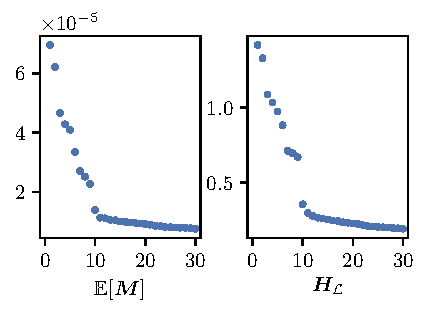
\includegraphics[width=0.25\linewidth]{Figures/EM_vs_H/LeNet5_fixlr0.01/UTAU_vs_full_sigval_d30_CIFAR10_Exp1_LeNet5_fixlr0.01R1_E-1_fc1.pdf}}
%     \qquad
%     \subfigure[\small{fc1:LeNet5 at min\\ (CIFAR10-R)}]{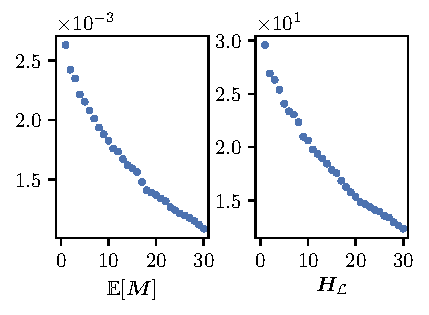
\includegraphics[width=0.25\linewidth]{Figures/EM_vs_H/LeNet5_RL/UTAU_vs_full_sigval_d30_CIFAR10_RandomLabel_LeNet5_fixlr0.01_RLR4_E-1_fc1.pdf}}
%     \caption{Eigenspectrum of the layer-wise output Hessian $\E[\mM]$ and the layer-wise weight Hessian $\mH_\Ls(\vw^{(p)})$. The vertical axes denote the eigenvalues. Similarity between the two eigenspectra is a direct consequence of a low rank $\E[\vx\vx^\T]$ and the decoupling conjecture.}
%     \label{fig:UTAU_H_spec}
%     \vspace{-2.5em}
% \end{figure}

% \subsection{Dominating Eigenvectors of Layer-wise Hessian are Low Rank}
% \label{sec:domin_eig}
% Here we verify the second prediction in \sectionref{sec:conjecture-implication}. From \figureref{fig:eigenvector-lowrank}
% for top eigenvector $\vh_i$, $\norm{\Mat(\vh_i)}$ is at least $\fn{\Mat(\vh_i)}/2$ (and often much larger), indicating the top eigenvectors of the layer-wise Hessians are very close to rank 1 after matricization.
% \begin{figure}[h]
% % \vskip -0.1in
% \centering
%     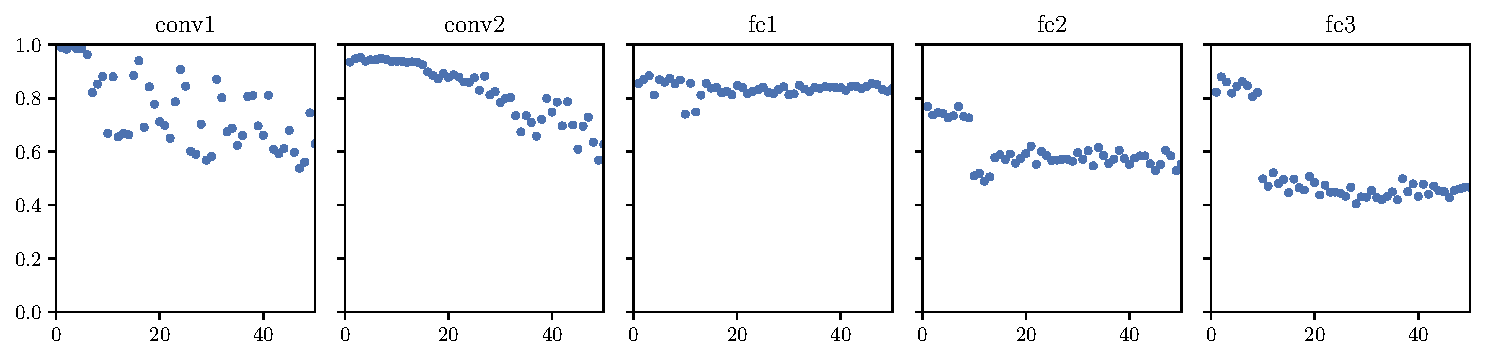
\includegraphics[width=0.75\columnwidth]{Figures/Eigenvec_Lowrank/NLeNet_base/5x1_Top_Eigenvector_rank_CIFAR10_Exp1_LeNet5_normnew_fixlr0.01R2_E-1_50.pdf}
%     %\captionsetup{justification=centering}
%     \vspace{-0.2in}
%     \caption{Ratio between top singular value and Frobenius norm of matricized dominating eigenvectors. (LeNet5 on CIFAR10). The horizontal axes denote the index $i$ of eigenvector $\vh_i$, and the vertical axes denote $\|\Mat(\vh_i)\|/\|\Mat(\vh_i)\|_F$.}
%     \label{fig:eigenvector-lowrank}
%     \vspace{-2.5em}
% \end{figure}
%\figureref{fig:eigen_lowrank} shows first singular values of $\Mat(\vh_i)$ divided by its Frobenius Norm for $i$ from 1 to 200. We can see that the top eigenvectors of the layer-wise Hessians are very close to rank 1.
% \znote{This figure does not contain much information}
% \begin{figure}[h]
% % \vskip -0.1in
% \centering
%     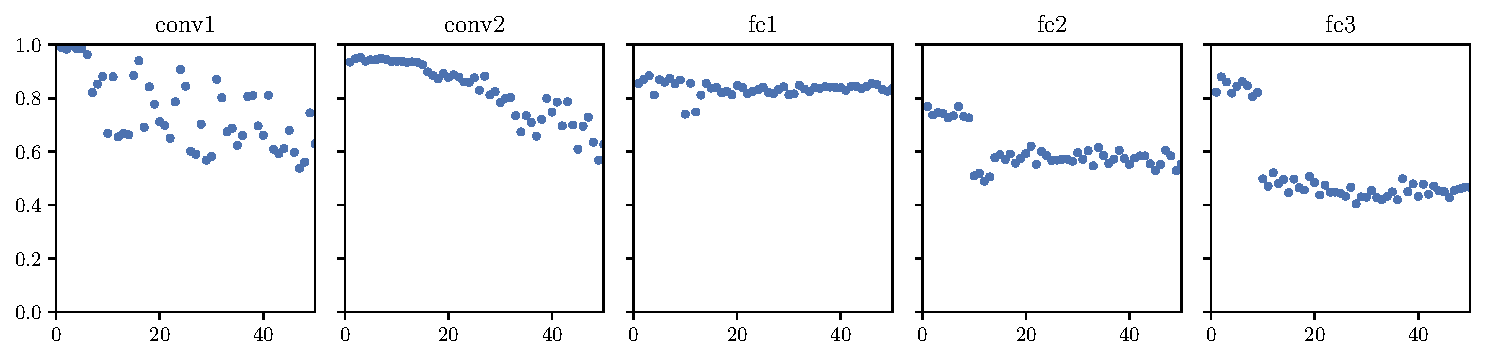
\includegraphics[width=0.75\columnwidth]{Figures/Eigenvec_Lowrank/NLeNet_base/5x1_Top_Eigenvector_rank_CIFAR10_Exp1_LeNet5_normnew_fixlr0.01R2_E-1_50.pdf}
%     %\captionsetup{justification=centering}
%     \vspace{-0.2in}
%     \caption{Ratio between top singular value and Frobenius norm of matricized dominating eigenvectors. (LeNet5 on CIFAR10). The horizontal axes denote the index $i$ of eigenvector $\vh_i$, and the vertical axes denote $\|\Mat(\vh_i)\|/\|\Mat(\vh_i)\|_F$.}
%     \label{fig:eigenvector-lowrank}
%     \vspace{-2.5em}
% \end{figure}

\subsection{Eigenspace Overlap of Different Models}
\label{sec:models}
Apart from the phenomena that are direct consequences of the decoupling conjecture, we observe another nontrivial phenomenon involving different minima.
Consider models with the same structure, trained on the same dataset, but using different random initializations, despite no obvious correlation between their parameters, we observe surpisingly high overlap between the dominating eigenspace of some of their layer-wise Hessians.
% \begin{figure}[h]
% \centering
% % \vspace{-1em}
% \subfigure[\small{conv12:ResNet18} ]{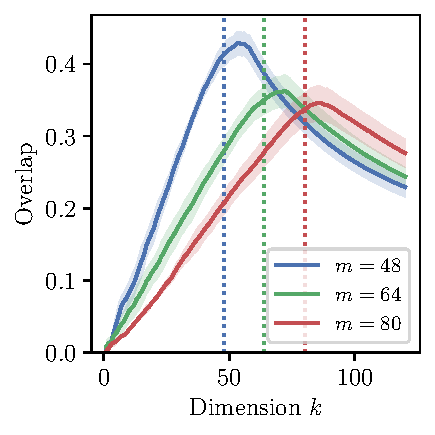
\includegraphics[width=0.25\linewidth]{Figures/SubspaceOverlap/NeurIPS/Overlap_ResNet_conv12.conv1.pdf}}
% \quad
% \subfigure[\small{conv6:VGG11} ]{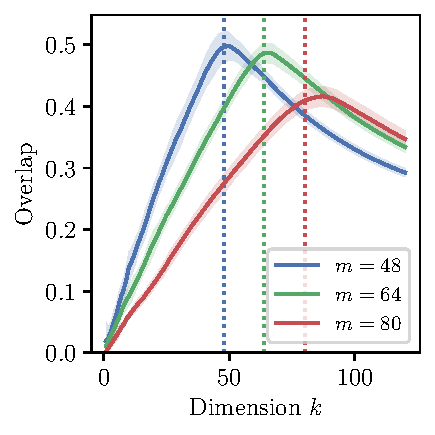
\includegraphics[width=0.25\linewidth]{Figures/SubspaceOverlap/NeurIPS/VGG11_conv6.pdf}}
% \quad
% \subfigure[\small{fc1:LeNet5} ]{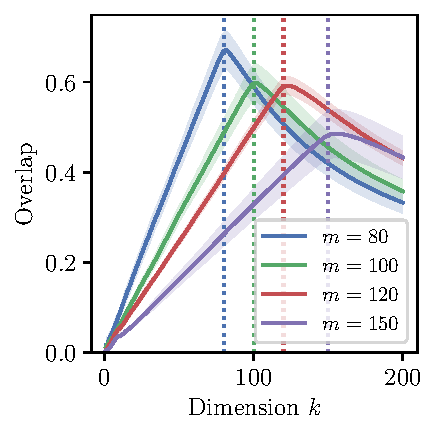
\includegraphics[width=0.25\linewidth]{Figures/SubspaceOverlap/NeurIPS/LeNetVarying.pdf}}
% \caption{Overlap between the top $k$ dominating eigenspace of different independently trained models. In each figure, we vary the number of output neuron/channels $m$. We includes 4 variants of LeNet5 trained on CIFAR10 (a), 3 variants of ResNet18 trained on CIFAR100 (b), and 3 different of VGG11 trained on CIFAR100 (c). For each structural variant, 5 models are trained from independent random initializations. We plot the average pairwise overlap between the top eigenspaces of those models' layer-wise Hessians. The overlap peaks at the output dimension $m$.}
% \label{fig:overlap}
% \vspace{-1em}
% \end{figure}


\begin{figure}[H]
    \captionsetup[sub]{format=subcaptionformat}
    \centering
    \begin{subfigure}[h]{0.32\columnwidth}
        \centering
        \captionsetup{justification=centering}
        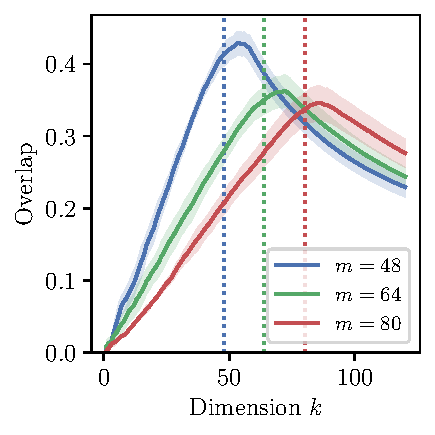
\includegraphics[width=\textwidth]{Figures/SubspaceOverlap/NeurIPS/Overlap_ResNet_conv12.conv1.pdf}
        \vspace{-0.2in}
        \caption{conv12:ResNet18 (CIFAR100) with 48/64/80 output channels}

        \label{fig:Overlap_resnet_conv1}
    \end{subfigure}
    \begin{subfigure}[h]{0.32\columnwidth}
        \centering
        \captionsetup{justification=centering}
        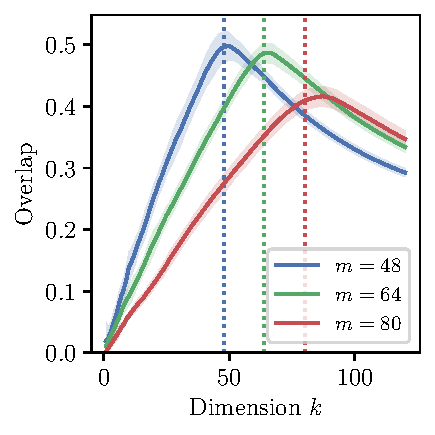
\includegraphics[width=\textwidth]{Figures/SubspaceOverlap/NeurIPS/VGG11_conv6.pdf}
        \vspace{-0.2in}
        \caption{conv6:VGG11 (CIFAR100) with 48/64/80 output channels}

        \label{fig:Overlap_resnet_conv2}
    \end{subfigure}
    \begin{subfigure}[h]{0.32\columnwidth}
        \centering
        \captionsetup{justification=centering}
        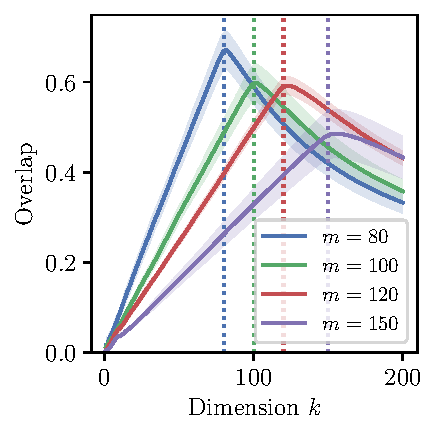
\includegraphics[width=\textwidth]{Figures/SubspaceOverlap/NeurIPS/LeNetVarying.pdf}
        \vspace{-0.2in}
        \caption{fc1:LeNet5 (CIFAR10) with 80/100/120/150 output neurons}

        \label{fig:Overlap_fc1}
    \end{subfigure}
    %\captionsetup{justification=centering}

    \caption{Overlap between the top $k$ dominating eigenspace of different independently trained models. The overlap peaks at the output dimension $m$. The eigenspace overlap is defined in \cref{def:overlap}.}
    \label{fig:overlap}
    \vskip -0.1in
\end{figure}

It turns out that the nontrivial overlap is also a consequence of the decoupling conjecture, which arises when the output Hessian and autocorrelation are related in the following way: When the small eigenvalues of $\E[\mM]\in\R^{m\times m}$ approaches 0 slower than the small eigenvalues of $\E[\vx\vx^\T]$, the top $m$ eigenspace will then be approximately spanned by $\mI_m\otimes \E[\vx]^\T$ by the decoupling conjecture.
Now suppose we have two different models with $\hE[\vx]_1$ and $\hE[\vx]_2$ respectively. Their top-$m$ eigenspaces are approximately $\mI_m \otimes \hE[\vx]_1$ and $\mI_m \otimes \hE[\vx]_2$. Thus the overlap at dimension $m$ is approximately $(\hE[\vx]_1^\T \hE[\vx]_2)^2$, which is large since $\hE[\vx]_1$ and $\hE[\vx]_2$ are the same for the input layer and all non-negative for other layers.
While this particular relation between $\E[\mM]$ and $\E[\vx\vx^\T]$ are true in many shallow networks and in later layers of deeper networks, they are not satisfied for earlier layers of deeper networks.  In \sectionref{sec:appendix_model_overlap} we explain how one can still understand the overlap using correspondence matrices when the above simplified argument does not hold. %why the overlap before rank-$m$ grows linearly. We also make a more general explanation and account for some cases where this argument does not hold. 

%Note that fc3 does not have the linear growth since neurons cannot be permuted in the last layer. \ynote{In addition, for the first layer, models with the same dataset would have the same $\hE[\vx]$, and that would lead to an overlap close to 1 at dimension $n$. Omit since we did not show the first layer}

%Then, consider the $(m+1)$th eigenvector of the first model. Since top $n$ eigenvectors span the full space $\Krsp(\hE[\vx]_1)$, it will be orthogonal to this space. It will also have low overlap with $\Krsp(\hE[\vx]_2)$ since $(\hE[\vx]_1 \cdot \hE[\vx]_2)$ is large. This explains the immediate drop in eigenspace overlap at dimension $m+1$. \ynote{May not be necessary}

% \subsection{Batch Normalization and Zero-mean Input}
% \snote{The approximation worsen, but is still relevant. Reason of low overlap: low correlation between $x$ in different layers, random permutation of neurons in FC layers.}
% According to our explanation, the good approximation and high overlap of top eigenspace both depend on the low rank structure of $\E[\vx\vx^T]$. Also, the low rank structure is caused by the fact that $\E[\vx]\E[\vx]^T$ dominates $\mSigma_\vx$ in most cases. Therefore, it's natural to conjecture that models trained using Batch Normalization (BN) \citep{ioffe2015batch} will change these phenomena as $\E[\vx]$ will be zero and $\E[\vx\vx^T] = \mSigma_\vx$ for those models. Indeed, as shown in \citet{ghorbani2019investigation}, BN suppresses the outliers in the Hessian eigenspectrum and \citet{papyan2020traces} provided an explanation.

% We experiment on our networks with BN. The results are shown in \sectionref{sec:appendix_batchnorm}. We found that $\E[\vx\vx^T]$ is no longer close to rank 1 for models trained with BN. However, $\E[\vx\vx^T]$ still have a few large eigenvalues. % and is not similar to a random matrix.
% In this case, all the previous structures ($c$ outliers, high eigenspace overlap, low rank eigenvectors) become weaker. The decoupling conjecture itself also becomes less accurate. However, the approximation still gives meaningful information. %our approximation in \sectionref{sec:approx_top_eig} is not accurate. Thus, the overlap of top $k$ eigenspace between different models can no longer be approximated as in \cref{eqn:model_overlap}. As expected, models with BN give a much lower eigenspace overlap at dimension smaller than $n$ and there is no obvious peak.

%The approximation of Hessian eigenvalues using Kronecker factorization is also not so accurate in models using BN, agreeing with our conjecture. However, the approximation still gives meaningful information and the top eigenspace overlap between true and approximated hessian is still (). It is lower than the case without BN but much larger than the expected value for 2 random subspaces.

% \paragraph{Remark} \znote{Batchnorm}